% Built by scripts/09_jse_to_tex.R from docs/draft/draft_v4_jse.md (Journal of Sports Economics / APA 7 layout).
% Compile from docs/draft: pdflatex draft_v4_jse.tex (twice).
\documentclass[12pt]{article}
\usepackage[margin=1in]{geometry}
\usepackage{mathptmx}
\usepackage[T1]{fontenc}\usepackage[utf8]{inputenc}
\usepackage{amsmath,amssymb}
\usepackage{booktabs,threeparttable,graphicx,float,array}
\usepackage{setspace}\doublespacing
\usepackage{endnotes}\renewcommand{\notesname}{Footnotes}
\usepackage{caption}
\captionsetup[table]{labelsep=newline,labelfont=bf,textfont=it,justification=raggedright,singlelinecheck=false,font=doublespacing}
\captionsetup[figure]{labelsep=period,labelfont=it,justification=raggedright,singlelinecheck=false,font=doublespacing}
\usepackage{hanging}
\usepackage[hidelinks]{hyperref}\usepackage{xurl}
\emergencystretch 3em
\setlength{\parindent}{0.5in}
\newcommand{\lone}[1]{\par\medskip\noindent\begin{center}\textbf{#1}\end{center}\par\nopagebreak}
\newcommand{\ltwo}[1]{\par\medskip\noindent\textbf{#1}\par\nopagebreak}
\newcommand{\lthree}[1]{\par\noindent\hspace{\parindent}\textbf{#1.}\ }
\pagestyle{plain}
\begin{document}

\begin{center}\textbf{
A Bright Line That Binds on Few: The NBA's 65-Game Rule and Star Availability
}\\[1em] Supplementary material\end{center}
\setcounter{table}{0}\renewcommand{\thetable}{A\arabic{table}}
\setcounter{figure}{0}\renewcommand{\thefigure}{A\arabic{figure}}
\lone{Appendix A. Additional Tables and Figures}
\noindent Tables A1 to A19 and Figures A1 to A3 are referenced in the text of the main manuscript. Table and figure sources are listed in the Markdown source of the manuscript.\clearpage
\begin{table}[!h]
\centering
\caption{\label{tab:tab4a_bunching_bins}Star player-seasons around the 65-game threshold, pre- vs post-rule}
\centering
\resizebox{\ifdim\width>\linewidth\linewidth\else\width\fi}{!}{
\begin{threeparttable}
\begin{tabular}[t]{lrlrl}
\toprule
Qualifying games & Pre: n & Pre: share & Post: n & Post: share\\
\midrule
<58 & 95 & 0.291 & 42 & 0.318\\
58-64 (below) & 40 & 0.122 & 15 & 0.114\\
65-68 (just above) & 41 & 0.125 & 14 & 0.106\\
69+ & 151 & 0.462 & 61 & 0.462\\
\bottomrule
\end{tabular}
\begin{tablenotes}
\item \textit{Note: } 
\item Stars, 2020-2021 excluded. Pre-rule 2014-2019 and 2022-2023; post-rule 2024-2026.
\end{tablenotes}
\end{threeparttable}}
\end{table}

\clearpage
\begin{table}[!h]
\centering
\caption{\label{tab:tab5a_at_risk_reach}Healthy at-risk stars at team game 62: did they reach 65?}
\centering
\resizebox{\ifdim\width>\linewidth\linewidth\else\width\fi}{!}{
\begin{threeparttable}
\begin{tabular}[t]{lrlrll}
\toprule
Slack at game 62 & Pre: n & Pre: reached 65 & Post: n & Post: reached 65 & Fisher p\\
\midrule
0-2 & 20 & 0.40 & 2 & 1.00 & 0.19\\
3-5 & 27 & 0.70 & 8 & 0.62 & 0.69\\
6-8 & 25 & 0.60 & 11 & 0.64 & 1.00\\
\bottomrule
\end{tabular}
\begin{tablenotes}
\item \textit{Note: } 
\item At risk: 0-8 games of slack at team game 62 (qualifying games so far plus games left minus 65). Healthy: played at least two of games 60-62. Reached: >= 65 qualifying games at season end. Fisher exact test of pre vs post.
\end{tablenotes}
\end{threeparttable}}
\end{table}

\clearpage
\begin{table}[!h]
\centering
\caption{\label{tab:tab5b_at_risk_regressions}Post-rule change in the probability that an at-risk star reaches 65}
\centering
\resizebox{\ifdim\width>\linewidth\linewidth\else\width\fi}{!}{
\begin{threeparttable}
\begin{tabular}[t]{lrrllll}
\toprule
Sample & n & Post n & Pre reach & Post reach & Post: est (SE) & MDE\\
\midrule
All at-risk stars & 116 & 34 & 0.56 & 0.53 & -0.05 (0.10) & 0.28\\
Healthy at game 62 & 93 & 21 & 0.58 & 0.67 & 0.06 (0.13) & 0.35\\
Healthy, with current-season contention control & 93 & 21 & 0.58 & 0.67 & 0.14 (0.13) & 0.36\\
Healthy, slack 0-5 & 57 & 10 & 0.57 & 0.70 & 0.13 (0.17) & 0.48\\
\bottomrule
\end{tabular}
\begin{tablenotes}
\item \textit{Note: } 
\item Linear probability models with slack-bin controls; SEs clustered by player. MDE at 80\% power, in probability points.
\end{tablenotes}
\end{threeparttable}}
\end{table}

\clearpage
\begin{table}[!h]
\centering
\caption{\label{tab:tab6b_absence_state_regressions}State x post-rule regressions of late-season absence, stars}
\centering
\resizebox{\ifdim\width>\linewidth\linewidth\else\width\fi}{!}{
\begin{threeparttable}
\begin{tabular}[t]{lllll}
\toprule
Specification & Term & Est (SE) & p & MDE\\
\midrule
state main effects + state x post & secured & 0.006 (0.013) & 0.61 & 0.036\\
state main effects + state x post & secured x post & -0.011 (0.019) & 0.56 & 0.053\\
no-incentive + no-incentive x post & no incentive & -0.004 (0.012) & 0.73 & 0.034\\
no-incentive + no-incentive x post & no incentive x post & -0.005 (0.019) & 0.78 & 0.053\\
\bottomrule
\end{tabular}
\begin{tablenotes}
\item \textit{Note: } 
\item Player-season and team-game-number fixed effects; SEs clustered by player. Reference state: reachable. MDE at 80\% power. The unreachable state is omitted: within a player-season its games follow a long absence, so the within-player contrast is mechanically negative and the post interaction is identified from few transitions; Table 6a carries that state.
\end{tablenotes}
\end{threeparttable}}
\end{table}

\clearpage
\begin{table}[!h]
\centering
\caption{\label{tab:tabA1_absence_event_study}Star minus non-star late-season absence by season}
\centering
\resizebox{\ifdim\width>\linewidth\linewidth\else\width\fi}{!}{
\begin{threeparttable}
\begin{tabular}[t]{rllllll}
\toprule
Season & Full, ref 2023: est (SE) & MDE & Full, ref 2017: est (SE) & MDE  & ESPN rows only, ref 2023: est (SE) & MDE  \\
\midrule
2014 & NA & NA & NA & NA & 0.023 (0.014) & 0.038\\
2015 & 0.010 (0.020) & 0.057 & 0.008 (0.019) & 0.054 & 0.009 (0.014) & 0.040\\
2016 & 0.001 (0.022) & 0.062 & -0.002 (0.021) & 0.058 & 0.023 (0.015) & 0.041\\
2017 & 0.006 (0.018) & 0.049 & 0.000 (0.000) & 0.000 & 0.018 (0.012) & 0.034\\
2018 & 0.005 (0.020) & 0.056 & 0.003 (0.019) & 0.053 & -0.002 (0.011) & 0.032\\
2019 & 0.035 (0.022) & 0.062 & 0.033 (0.022) & 0.061 & -0.001 (0.015) & 0.043\\
2022 & 0.031 (0.020) & 0.057 & 0.029 (0.021) & 0.060 & 0.012 (0.013) & 0.036\\
2023 & 0.000 (0.000) & 0.000 & -0.008 (0.021) & 0.059 & 0.000 (0.000) & 0.000\\
2024 & -0.008 (0.018) & 0.050 & -0.010 (0.020) & 0.055 & -0.009 (0.008) & 0.023\\
2025 & -0.017 (0.025) & 0.069 & -0.019 (0.026) & 0.074 & -0.005 (0.014) & 0.039\\
2026 & -0.018 (0.024) & 0.068 & -0.020 (0.025) & 0.071 & -0.021 (0.010) & 0.029\\
\bottomrule
\end{tabular}
\begin{tablenotes}
\item \textit{Note: } 
\item Coefficients on star x season; player, season and team-game-number fixed effects; SEs clustered by player. 'ESPN rows only' reproduces the exploratory construction in which only games with an ESPN row enter.
\end{tablenotes}
\end{threeparttable}}
\end{table}

\clearpage
\begin{table}[!h]
\centering
\caption{\label{tab:tabA3_long_absences}Spells of 10 or more consecutive missed games, stars and high-minute non-stars}
\centering
\resizebox{\ifdim\width>\linewidth\linewidth\else\width\fi}{!}{
\begin{threeparttable}
\begin{tabular}[t]{llrrllllllllllll}
\toprule
Group & Period & Player-seasons & Spells & Spells per star-season & Star-seasons with a spell & Mean length & Games lost per star-season & Censored at season end & Reason: injury/illness & Reason: no row & Reason: rest or coach & Begin games 1-20 & 21-40 & 41-55 & 56-82\\
\midrule
Stars & Pre-rule & 327 & 127 & 0.39 & 33\% & 25.6 & 10.0 & 31\% & 30\% & 56\% & 11\% & 35\% & 25\% & 18\% & 21\%\\
Stars & Post-rule & 132 & 65 & 0.49 & 39\% & 22.2 & 11.0 & 34\% & 20\% & 77\% & 0\% & 34\% & 11\% & 25\% & 31\%\\
High-minute non-stars (prior season) & Pre-rule & 542 & 213 & 0.39 & 34\% & 24.0 & 9.4 & 39\% & 32\% & 54\% & 12\% & 38\% & 16\% & 14\% & 32\%\\
High-minute non-stars (prior season) & Post-rule & 239 & 111 & 0.46 & 38\% & 19.9 & 9.2 & 32\% & 32\% & 62\% & 3\% & 35\% & 25\% & 14\% & 26\%\\
\bottomrule
\end{tabular}
\begin{tablenotes}
\item \textit{Note: } 
\item Full team schedule, 2020-2021 excluded. Reason taken from the first game in the spell for which ESPN printed a row; 'no row' spells have no ESPN row at any point.
\end{tablenotes}
\end{threeparttable}}
\end{table}

\clearpage
\begin{table}[!h]
\centering
\caption{\label{tab:tabA8_composition_2024}Decomposition of the 2023 to 2024 change in mean games: stayers, entrants and leavers}
\centering
\resizebox{\ifdim\width>\linewidth\linewidth\else\width\fi}{!}{
\begin{threeparttable}
\begin{tabular}[t]{llllrlllll}
\toprule
Outcome & Mean 2023 (n) & Mean 2024 (n) & Raw change & Stayers: n & Stayers 2023 & Stayers 2024 & Stayers change & Entrants 2024 (n) & Leavers 2023 (n)\\
\midrule
Stars: games played & 59.4 (45) & 65.0 (46) & 5.6 & 39 & 61.3 & 64.2 & 2.9 & 69.6 (7) & 46.7 (6)\\
Stars: qualifying games & 58.4 (45) & 64.5 (46) & 6.1 & 39 & 60.6 & 63.7 & 3.0 & 69.3 (7) & 44.2 (6)\\
High-minute non-stars (prior season): games played & 65.6 (82) & 66.1 (90) & 0.6 & 50 & 69.7 & 66.0 & -3.8 & 66.4 (40) & 59.1 (32)\\
\bottomrule
\end{tabular}
\begin{tablenotes}
\item \textit{Note: } 
\item Stayers are players in the group in both seasons; entrants are 2024 members who were not members in 2023; leavers are 2023 members who were not members in 2024. The within-player event-study coefficient is identified from stayers.
\end{tablenotes}
\end{threeparttable}}
\end{table}

\clearpage
\begin{table}[!h]
\centering
\caption{\label{tab:tabA9_cohort_pairs}Fixed-cohort difference-in-differences for each pair of adjacent seasons, games played}
\centering
\resizebox{\ifdim\width>\linewidth\linewidth\else\width\fi}{!}{
\begin{threeparttable}
\begin{tabular}[t]{lrlrllll}
\toprule
Seasons & Stars (n) & Stars: first, second & Controls (n) & Controls: first, second & DiD: est (SE) & p & MDE\\
\midrule
2015->2016 & 42 & 64.7, 67.5 & 85 & 66.3, 65.0 & 4.15 (3.77) & 0.27 & 10.6\\
2016->2017 & 42 & 70.5, 69.0 & 69 & 67.4, 66.2 & -0.31 (3.06) & 0.92 & 8.6\\
2017->2018 & 39 & 70.8, 63.3 & 74 & 66.2, 62.2 & -3.59 (3.89) & 0.36 & 10.9\\
2018->2019 & 36 & 64.2, 63.3 & 72 & 63.9, 63.3 & -0.31 (5.16) & 0.95 & 14.5\\
2022->2023 & 38 & 58.4, 60.1 & 73 & 61.1, 63.7 & -0.92 (3.93) & 0.82 & 11.0\\
2023->2024 & 44 & 60.5, 63.3 & 80 & 65.8, 63.9 & 4.66 (3.44) & 0.18 & 9.6\\
2024->2025 & 46 & 65.0, 63.0 & 86 & 66.9, 61.0 & 3.91 (3.32) & 0.24 & 9.3\\
2025->2026 & 43 & 62.5, 52.9 & 79 & 61.5, 57.0 & -5.16 (4.64) & 0.27 & 13.0\\
\bottomrule
\end{tabular}
\begin{tablenotes}
\item \textit{Note: } 
\item Groups fixed at their status in the first season of the pair; players present in both seasons; player and season fixed effects; SEs clustered by player. The 2023 to 2024 row is the year the rule took effect.
\end{tablenotes}
\end{threeparttable}}
\end{table}

\clearpage
\begin{table}[!h]
\centering
\caption{\label{tab:tabA10_bound_windows}The maximal-effect bound under alternative definitions of the at-risk population}
\centering
\resizebox{\ifdim\width>\linewidth\linewidth\else\width\fi}{!}{
\begin{threeparttable}
\begin{tabular}[t]{rlllllll}
\toprule
Slack measured at game & Window & Period & At risk per season & Share of stars & Did not reach & Bound, minimal crossing & Bound, play every game\\
\midrule
55 & 0-12 & Pre-rule & 16.8 & 0.41 & 6.0 & 1.07 & 2.42\\
55 & 0-12 & Post-rule & 20.7 & 0.47 & 7.3 & 1.71 & 3.79\\
55 & 0-8 & Pre-rule & 9.5 & 0.23 & 4.6 & 0.89 & 1.55\\
55 & 0-8 & Post-rule & 9.7 & 0.22 & 5.3 & 1.30 & 2.10\\
62 & 0-12 & Pre-rule & 17.9 & 0.44 & 5.4 & 0.75 & 2.05\\
62 & 0-12 & Post-rule & 20.3 & 0.46 & 5.7 & 0.99 & 2.55\\
62 & 0-8 & Pre-rule & 10.2 & 0.25 & 4.5 & 0.67 & 1.28\\
62 & 0-8 & Post-rule & 11.3 & 0.26 & 5.3 & 0.98 & 1.83\\
\bottomrule
\end{tabular}
\begin{tablenotes}
\item \textit{Note: } 
\item Same construction as Table 5c with slack measured at team game 62 or 55 and the window widened to 0-12 games.
\end{tablenotes}
\end{threeparttable}}
\end{table}

\clearpage
\begin{table}[!h]
\centering
\caption{\label{tab:tabA11_exact65}Finishing at exactly 65 qualifying games among stars who reached the line}
\centering
\resizebox{\ifdim\width>\linewidth\linewidth\else\width\fi}{!}{
\begin{threeparttable}
\begin{tabular}[t]{llrrlll}
\toprule
Sample & Period & n & Finished at exactly 65 & Share & Mean final qualifying games & Fisher p\\
\midrule
all star reachers & Pre-rule & 192 & 9 & 0.05 & 73.7 & 0.16\\
all star reachers & Post-rule & 75 & 7 & 0.09 & 72.7 & 0.16\\
at-risk reachers & Pre-rule & 46 & 8 & 0.17 & 67.3 & 0.19\\
at-risk reachers & Post-rule & 18 & 6 & 0.33 & 67.8 & 0.19\\
healthy at-risk reachers & Pre-rule & 42 & 8 & 0.19 & 67.1 & 0.27\\
healthy at-risk reachers & Post-rule & 14 & 5 & 0.36 & 67.9 & 0.27\\
\bottomrule
\end{tabular}
\begin{tablenotes}
\item \textit{Note: } 
\item At-risk: 0-8 games of slack at team game 62. Healthy: played at least two of games 60-62. Fisher exact test of pre vs post within sample.
\end{tablenotes}
\end{threeparttable}}
\end{table}

\clearpage
\begin{table}[!h]
\centering
\caption{\label{tab:tabA11b_exact65_distribution}Final qualifying games of at-risk stars who reached 65}
\centering
\resizebox{\ifdim\width>\linewidth\linewidth\else\width\fi}{!}{
\begin{tabular}[t]{lrlrl}
\toprule
Final qualifying games & Pre: n & Pre: share & Post: n & Post: share\\
\midrule
65 & 8 & 0.17 & 6 & 0.33\\
66 & 13 & 0.28 & 0 & 0.00\\
67 & 7 & 0.15 & 2 & 0.11\\
68 & 8 & 0.17 & 3 & 0.17\\
69 & 3 & 0.07 & 1 & 0.06\\
70 & 2 & 0.04 & 4 & 0.22\\
71 & 3 & 0.07 & 1 & 0.06\\
72 & 2 & 0.04 & 1 & 0.06\\
\bottomrule
\end{tabular}}
\end{table}

\clearpage
\begin{table}[!h]
\centering
\caption{\label{tab:tabA13_late_onset}Long absences beginning in the late-season window, before and after the rule}
\centering
\resizebox{\ifdim\width>\linewidth\linewidth\else\width\fi}{!}{
\begin{threeparttable}
\begin{tabular}[t]{llrrll}
\toprule
Group & Period & Spells & Beginning at game 56+ & Share & Fisher p (pre vs post)\\
\midrule
Stars & Pre-rule & 127 & 27 & 0.21 & 0.16\\
Stars & Post-rule & 65 & 20 & 0.31 & 0.16\\
High-minute non-stars (prior season) & Pre-rule & 213 & 69 & 0.32 & 0.25\\
High-minute non-stars (prior season) & Post-rule & 111 & 29 & 0.26 & 0.25\\
\bottomrule
\end{tabular}
\begin{tablenotes}
\item \textit{Note: } 
\item Difference in shares, stars minus control, post minus pre: 0.158 with bootstrap 95\% interval [-0.012, 0.329] from 2,000 resamples of spells within group and period.
\end{tablenotes}
\end{threeparttable}}
\end{table}

\clearpage
\begin{table}[!h]
\centering
\caption{\label{tab:tabA14_bbr_boxscore_check}ESPN box-score rows against Basketball-Reference did-not-play and inactive lists, sample games}
\centering
\resizebox{\ifdim\width>\linewidth\linewidth\else\width\fi}{!}{
\begin{threeparttable}
\begin{tabular}[t]{rlrrrrrrrll}
\toprule
Season & Game & ESPN rows & BBR box rows & ESPN rows found in BBR box & ESPN DNP rows & Of which BBR did-not-play & BBR inactive & BBR inactive with an ESPN row & Star with no ESPN row & On BBR inactive list\\
\midrule
2015 & 2014-12-03 & 26 & 68 & 26 & 6 & 6 & 3 & 0 & DeMar DeRozan & TRUE\\
2017 & 2016-12-28 & 26 & 68 & 26 & 7 & 7 & 4 & 0 & Damian Lillard & TRUE\\
2019 & 2018-11-15 & 25 & 67 & 25 & 4 & 4 & 8 & 0 & Pau Gasol & TRUE\\
2023 & 2023-01-31 & 28 & 70 & 28 & 8 & 8 & 6 & 0 & Zion Williamson & TRUE\\
2024 & 2024-01-15 & 25 & 67 & 25 & 7 & 7 & 9 & 0 & Jaylen Brown & TRUE\\
2025 & 2025-03-15 & 25 & 67 & 25 & 3 & 3 & 11 & 0 & Ja Morant & TRUE\\
2026 & 2026-03-07 & 26 & 68 & 26 & 5 & 5 & 10 & 0 & Jaren Jackson Jr. & TRUE\\
\bottomrule
\end{tabular}
\begin{tablenotes}
\item \textit{Note: } 
\item One game per season, chosen so that a star has an ESPN no-row absence. BBR box scores list did-not-play and did-not-dress players inside the box and inactive players below it.
\end{tablenotes}
\end{threeparttable}}
\end{table}

\clearpage
\begin{table}[!h]
\centering
\caption{\label{tab:tabA5_bbr_validation}Games played: ten star-seasons checked against Basketball-Reference}
\centering
\resizebox{\ifdim\width>\linewidth\linewidth\else\width\fi}{!}{
\begin{threeparttable}
\begin{tabular}[t]{rlrllllll}
\toprule
Season & Player & Reference games played & This paper: regular season & Raw ESPN count & Games under the rule (incl. Cup final) & Qualifying games & Status & Source\\
\midrule
2024 & Joel Embiid & 39 & 39 & 39 & 39 & 39 & match & web lookup 2026-09-15 (ESPN game log, StatMuse); BBR not re-requested\\
2024 & Tyrese Haliburton & 69 & 69 & 71 & 70 & 69 & match & cached BBR awards\_2024.html (MIP and All-NBA voting tables, G column)\\
2023 & Stephen Curry & 56 & 56 & 56 & 56 & 56 & match & cached BBR awards\_2023.html (MVP voting table, G column)\\
2025 & Luka Doncic & 50 & 50 & 50 & 50 & 50 & match & web lookup 2026-09-15 (22 DAL + 28 LAL); BBR not re-requested\\
2024 & Nikola Jokic & 79 & 79 & 80 & 79 & 79 & match & cached BBR awards\_2024.html (MVP voting table, G column)\\
2023 & LeBron James & 55 & 55 & 56 & 55 & 55 & match & cached BBR awards\_2023.html (All-NBA voting table, G column)\\
2022 & Kawhi Leonard & 0 &  &  &  &  & no ESPN rows; not in sample & missed the entire 2021-22 season (ACL); web lookup 2026-09-15\\
2024 & Jimmy Butler & 60 & 60 & 60 & 60 & 60 & match & web lookup 2026-09-15; BBR not re-requested\\
2024 & Donovan Mitchell & 55 & 55 & 56 & 55 & 55 & match & web lookup 2026-09-15 (StatMuse); BBR not re-requested\\
2026 & Victor Wembanyama & 64 & 64 & 67 & 65 & 65 & match & cached BBR awards\_2026.html (MVP, DPOY, All-NBA voting tables, G column)\\
\bottomrule
\end{tabular}
\begin{tablenotes}
\item \textit{Note: } 
\item Reference values from cached Basketball-Reference award-voting tables where available, otherwise from a web lookup on the date shown. Regular-season games exclude the All-Star game and the NBA Cup final, as Basketball-Reference does; the rule's count includes the Cup final.
\end{tablenotes}
\end{threeparttable}}
\end{table}

\clearpage
\begin{table}[!h]
\centering
\caption{\label{tab:tabA7_exhibition_correction}Effect of removing All-Star and Rising Stars rows on star counts}
\centering
\resizebox{\ifdim\width>\linewidth\linewidth\else\width\fi}{!}{
\begin{threeparttable}
\begin{tabular}[t]{rrrrllllr}
\toprule
Season & Stars & GP changed & QG changed & Mean GP, raw & Mean GP, clean & Mean QG, raw & Mean QG, clean & Crossed 65 only via exhibition\\
\midrule
2014 & 41 & 18 & 10 & 60.7 & 60.3 & 58.2 & 57.9 & 0\\
2015 & 43 & 16 & 11 & 63.5 & 63.2 & 61.1 & 60.9 & 0\\
2016 & 46 & 20 & 16 & 69.5 & 69.1 & 66.4 & 66.0 & 0\\
2017 & 40 & 21 & 17 & 70.8 & 70.2 & 66.7 & 66.3 & 0\\
2018 & 36 & 18 & 15 & 64.7 & 64.2 & 62.6 & 62.2 & 0\\
2019 & 37 & 19 & 13 & 63.6 & 63.1 & 61.9 & 61.6 & 1\\
2022 & 39 & 15 & 10 & 58.5 & 58.1 & 56.9 & 56.7 & 0\\
2023 & 45 & 16 & 14 & 59.7 & 59.4 & 58.8 & 58.4 & 1\\
2024 & 46 & 19 & 14 & 65.5 & 65.0 & 64.8 & 64.5 & 0\\
2025 & 46 & 16 & 0 & 63.1 & 62.4 & 62.0 & 62.0 & 0\\
2026 & 40 & 18 & 0 & 56.1 & 54.8 & 54.4 & 54.4 & 0\\
\bottomrule
\end{tabular}
\begin{tablenotes}
\item \textit{Note: } 
\item Games played also exclude the NBA Cup final (a non-regular-season game for statistics); qualifying games include it, as the rule does.
\end{tablenotes}
\end{threeparttable}}
\end{table}

\clearpage
\begin{table}[!h]
\centering
\caption{\label{tab:tabA2_minute_bins}Minutes played by late-season stars, by slack: share of player-games (cell count)}
\centering
\resizebox{\ifdim\width>\linewidth\linewidth\else\width\fi}{!}{
\begin{threeparttable}
\begin{tabular}[t]{llllll}
\toprule
Sample & Minutes & pre, not tight & pre, tight & post, not tight & post, tight\\
\midrule
All & <15 & 0.018 (103) & 0.010 (7) & 0.007 (16) & 0.000 (0)\\
All & 15-19 & 0.030 (173) & 0.031 (22) & 0.010 (22) & 0.011 (2)\\
All & 20-22 & 0.037 (211) & 0.042 (30) & 0.026 (57) & 0.043 (8)\\
All & 23-30 & 0.243 (1385) & 0.294 (209) & 0.215 (470) & 0.368 (68)\\
All & 31+ & 0.671 (3823) & 0.623 (442) & 0.742 (1622) & 0.578 (107)\\
Played each of previous 3 games & <15 & 0.013 (58) & 0.013 (7) & 0.004 (7) & 0.000 (0)\\
Played each of previous 3 games & 15-19 & 0.021 (98) & 0.033 (17) & 0.009 (15) & 0.000 (0)\\
Played each of previous 3 games & 20-22 & 0.031 (142) & 0.034 (18) & 0.026 (43) & 0.034 (4)\\
Played each of previous 3 games & 23-30 & 0.239 (1090) & 0.295 (154) & 0.202 (340) & 0.325 (38)\\
Played each of previous 3 games & 31+ & 0.696 (3176) & 0.625 (326) & 0.759 (1275) & 0.641 (75)\\
\bottomrule
\end{tabular}
\begin{tablenotes}
\item \textit{Note: } 
\item Stars who played, games 56 onward, 2020-2021 excluded. Tight: 0-3 games of slack and 65 not yet secured. Cell counts in parentheses. Confounded by minute restrictions on players returning from injury.
\end{tablenotes}
\end{threeparttable}}
\end{table}

\clearpage
\begin{table}[!h]
\centering
\caption{\label{tab:tabA4_absence_reasons}What ESPN says about late-season absences of stars who played the previous game}
\centering
\resizebox{\ifdim\width>\linewidth\linewidth\else\width\fi}{!}{
\begin{threeparttable}
\begin{tabular}[t]{llrl}
\toprule
Period & Class & n & Share\\
\midrule
Pre-rule & no row (reason unknown) & 345 & 54.9\%\\
Pre-rule & injury or illness & 113 & 18.0\%\\
Pre-rule & coach's decision & 107 & 17.0\%\\
Pre-rule & rest & 52 & 8.3\%\\
Pre-rule & other & 11 & 1.8\%\\
Post-rule & no row (reason unknown) & 221 & 81.0\%\\
Post-rule & injury or illness & 41 & 15.0\%\\
Post-rule & rest & 7 & 2.6\%\\
Post-rule & other & 4 & 1.5\%\\
\bottomrule
\end{tabular}
\begin{tablenotes}
\item \textit{Note: } 
\item Classes from the DNP reason string. Absences with no ESPN row carry no reason.
\end{tablenotes}
\end{threeparttable}}
\end{table}

\clearpage
\begin{table}[!h]
\centering
\caption{\label{tab:tabA6_stars_no_appearance}Flagged stars absent from the sample: no ESPN box-score row in the season}
\centering
\resizebox{\ifdim\width>\linewidth\linewidth\else\width\fi}{!}{
\begin{threeparttable}
\begin{tabular}[t]{rl}
\toprule
Season & Flagged stars with no ESPN appearance\\
\midrule
2015 & Andrew Bynum\\
2017 & Chris Bosh; Kobe Bryant; Tim Duncan\\
2018 & Chris Bosh; Kobe Bryant; Tim Duncan\\
2019 & Kobe Bryant\\
2020 & Dirk Nowitzki; Dwyane Wade; John Wall; Kevin Durant; Klay Thompson\\
2021 & Dirk Nowitzki; Dwyane Wade; Klay Thompson\\
2022 & Dirk Nowitzki; Dwyane Wade; Kawhi Leonard; Zion Williamson\\
2026 & Kyrie Irving; Tyrese Haliburton\\
\bottomrule
\end{tabular}
\begin{tablenotes}
\item \textit{Note: } 
\item Retired players and players who missed the entire season. They do not enter any player-season count.
\end{tablenotes}
\end{threeparttable}}
\end{table}

\clearpage
\begin{table}[!h]
\centering
\caption{\label{tab:tabA16_rowsonly_raw}Late-season 'rest' rates computed on ESPN rows only (exploratory construction)}
\centering
\resizebox{\ifdim\width>\linewidth\linewidth\else\width\fi}{!}{
\begin{threeparttable}
\begin{tabular}[t]{rllrr}
\toprule
Season & Stars: share sat (ESPN rows only) & Contemporaneous control: share sat (ESPN rows only) & Star player-games & Control player-games\\
\midrule
2014 & 0.071 & 0.030 & 776 & 2301\\
2015 & 0.058 & 0.041 & 824 & 1721\\
2016 & 0.068 & 0.037 & 981 & 1809\\
2017 & 0.055 & 0.030 & 851 & 1773\\
2018 & 0.028 & 0.024 & 713 & 1630\\
2019 & 0.036 & 0.030 & 758 & 1693\\
2022 & 0.032 & 0.027 & 709 & 1834\\
2023 & 0.011 & 0.021 & 842 & 2110\\
2024 & 0.017 & 0.032 & 906 & 1739\\
2025 & 0.042 & 0.054 & 835 & 1372\\
2026 & 0.014 & 0.036 & 633 & 1486\\
\bottomrule
\end{tabular}
\begin{tablenotes}
\item \textit{Note: } 
\item Player-games with an ESPN row whose previous ESPN row was a game played, games 56 onward; the outcome is a did-not-play row. This construction omits inactive-list absences and tracks roster designation (Table 2); it is shown only to document the earlier numbers.
\end{tablenotes}
\end{threeparttable}}
\end{table}

\clearpage
\begin{figure}[p]
\centering
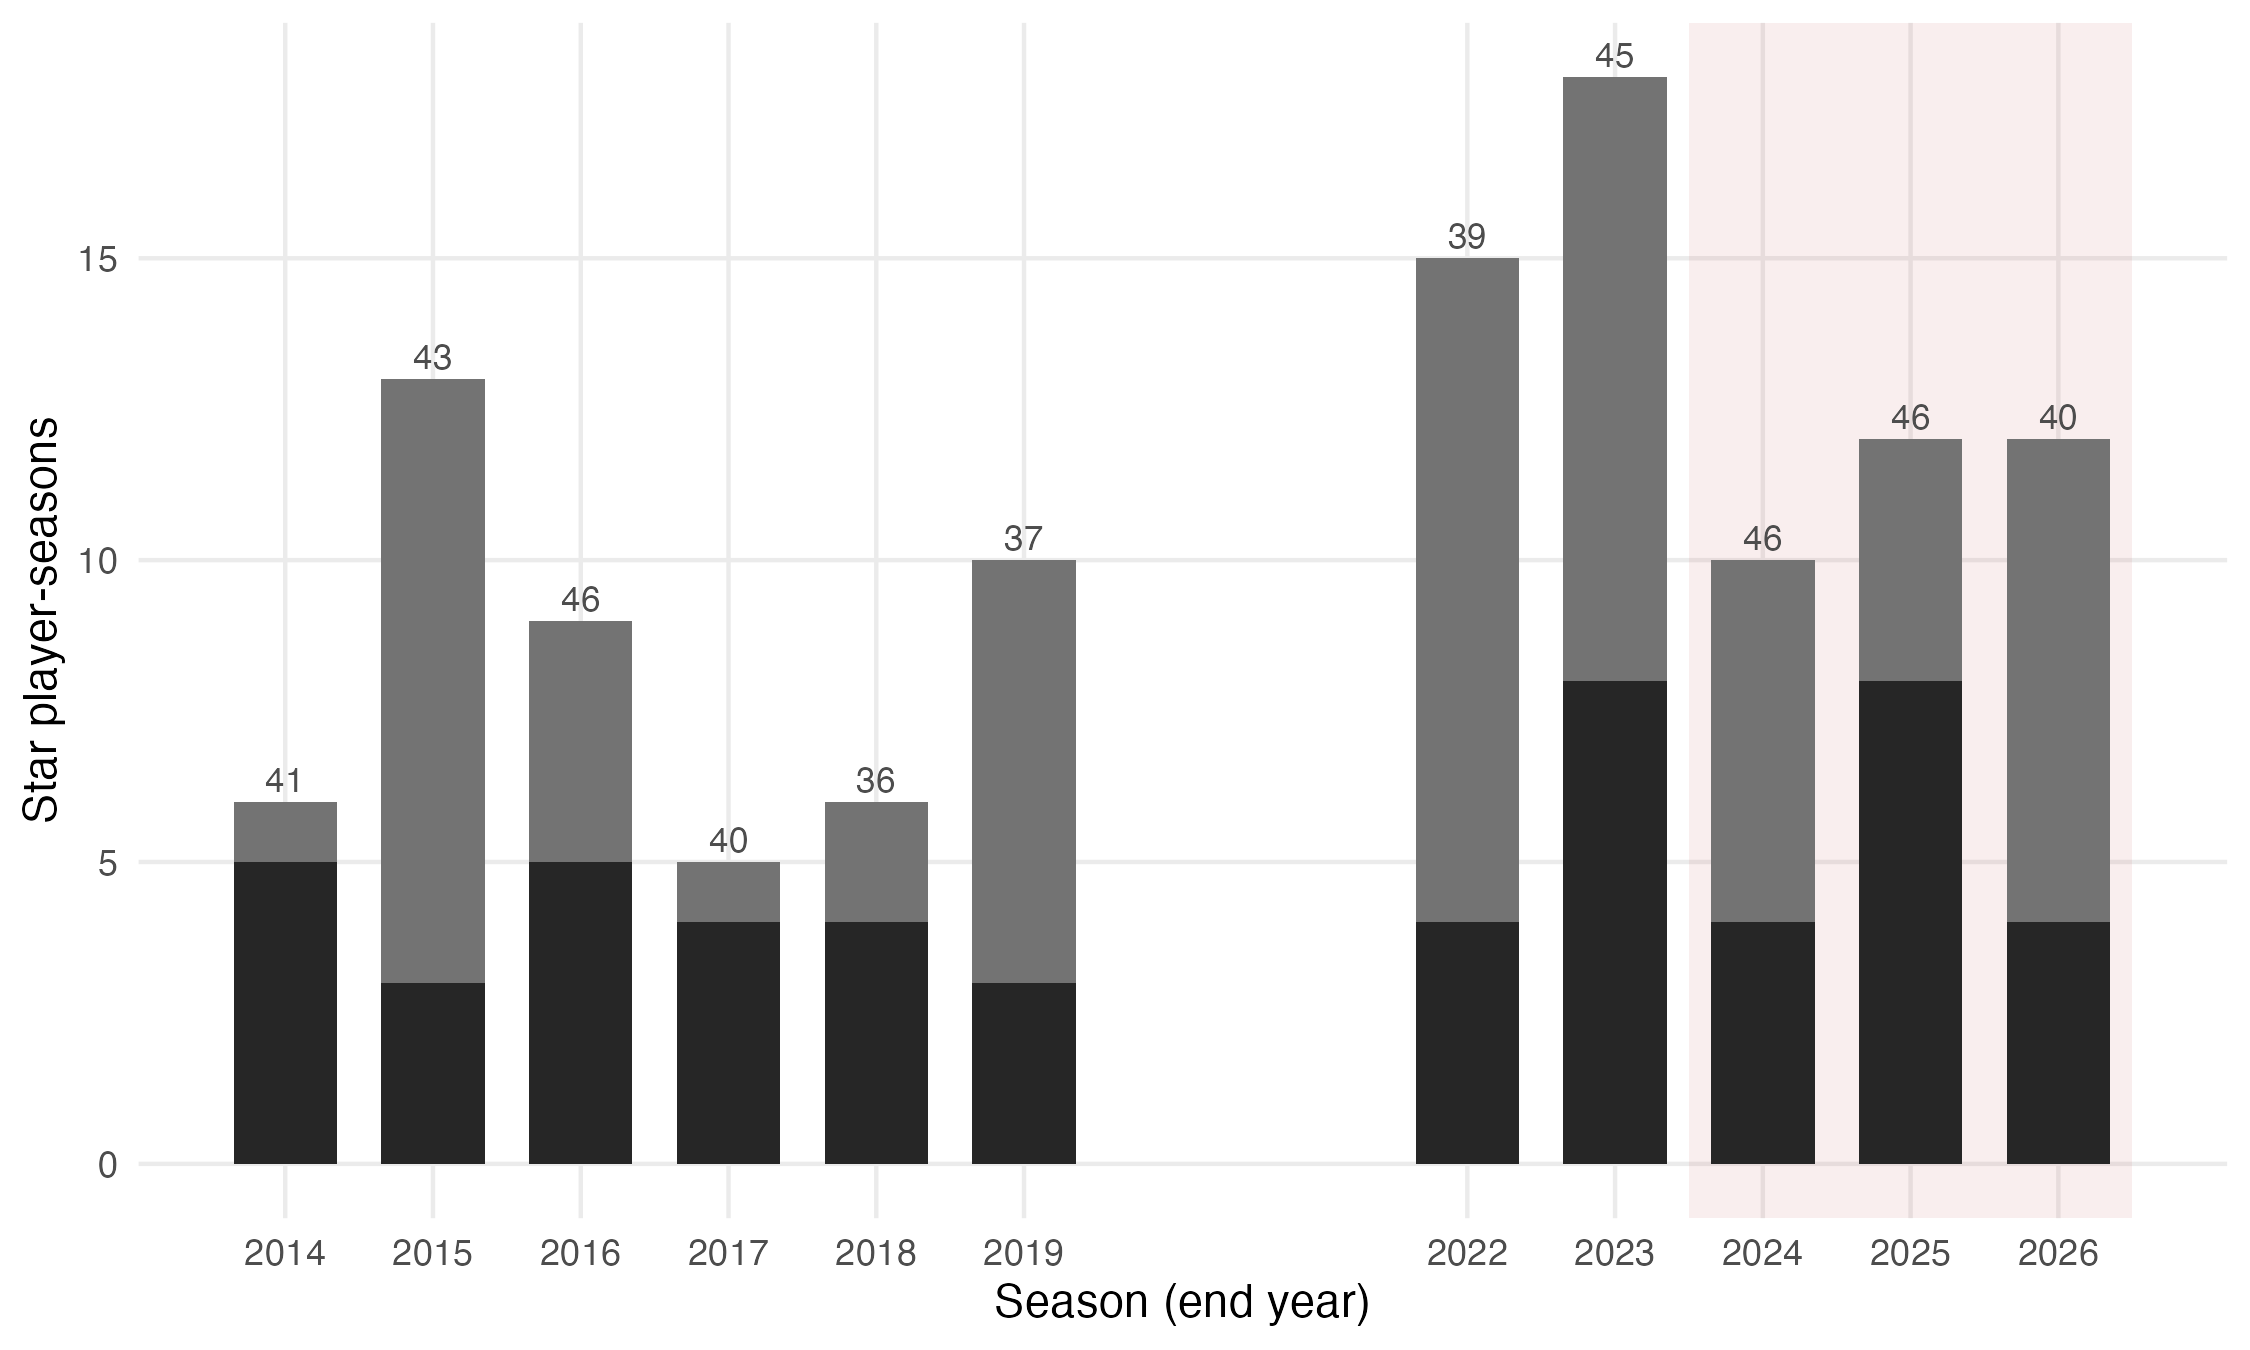
\includegraphics[width=\linewidth]{../../results/figures/paper/figA1_at_risk_by_season.png}
\caption{Stars at risk at team game 62 (slack 0-8), by season; black: at risk and did not reach 65; number above bar: stars that season.}
\end{figure}
\clearpage
\begin{figure}[p]
\centering
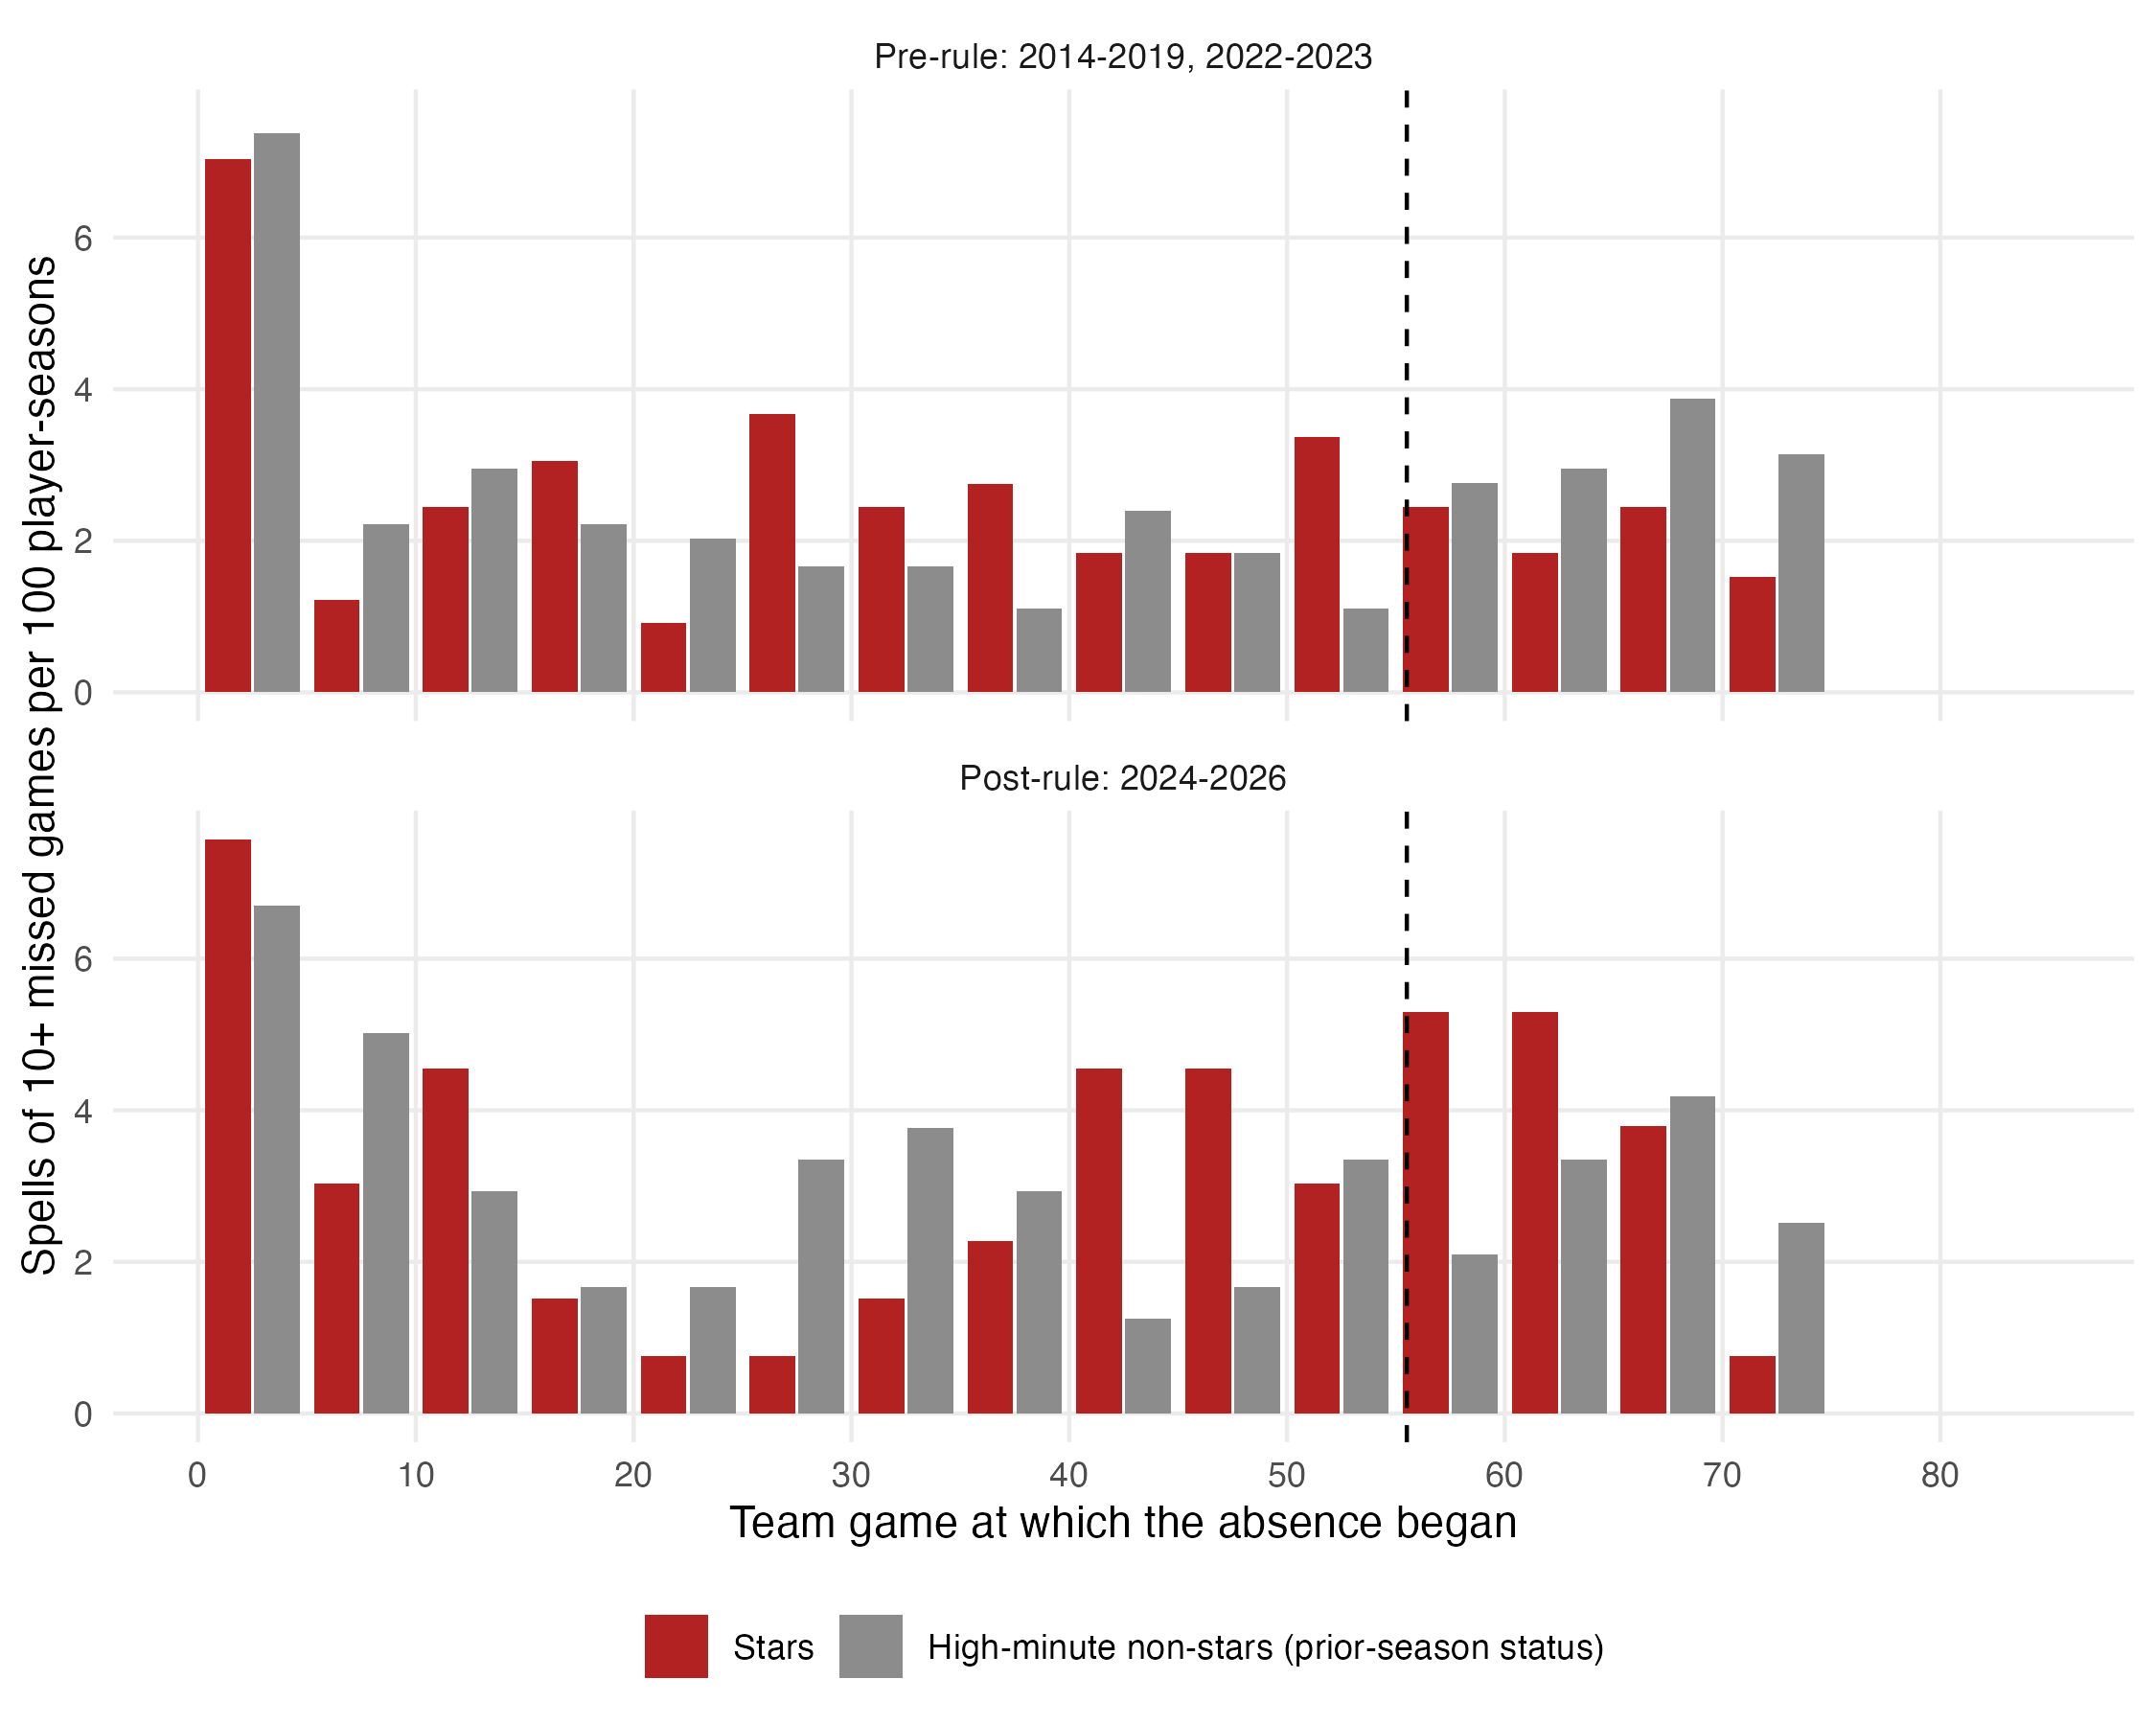
\includegraphics[width=\linewidth]{../../results/figures/paper/figA2_absence_timing.png}
\caption{Team game at which spells of 10 or more missed games began, per 100 player-seasons, stars and control, before and after the rule.}
\end{figure}
\clearpage
\begin{figure}[p]
\centering
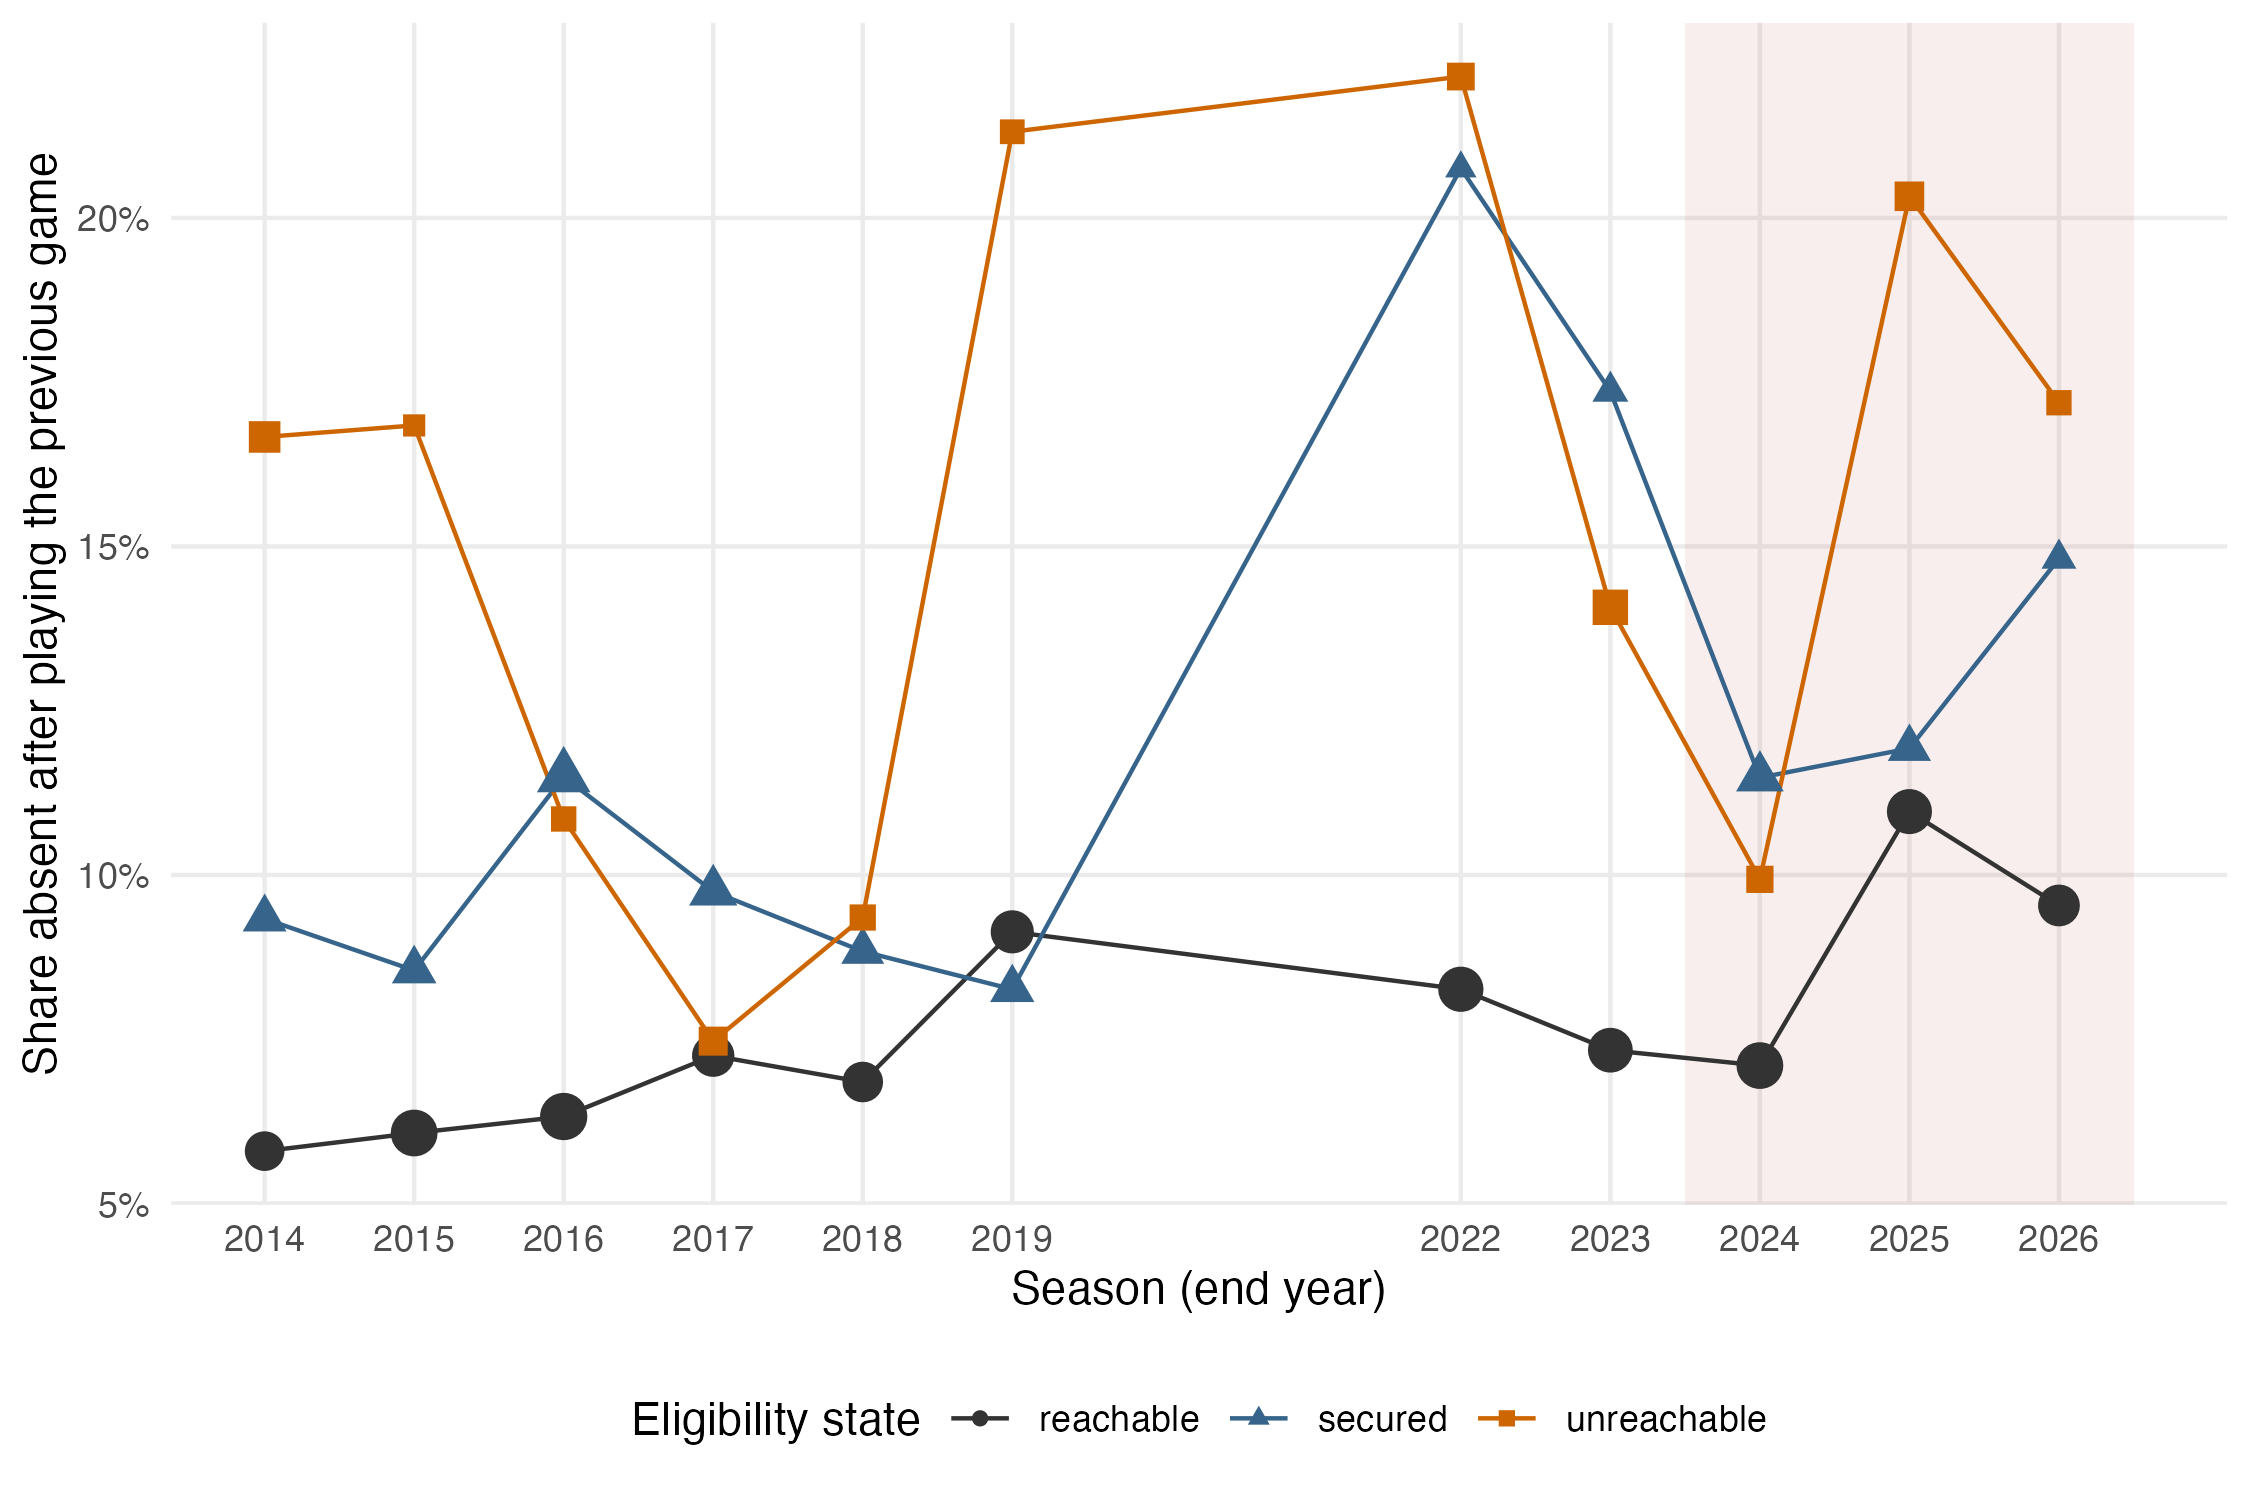
\includegraphics[width=\linewidth]{../../results/figures/paper/figA3_absence_by_state_by_season.png}
\caption{Late-season absence of stars who played the previous game, by eligibility state and season; point size is the number of player-games in the cell.}
\end{figure}
\clearpage
\end{document}
